\chapter{Fundamentação Teórica}\label{ch:fundamentacao}

A seguir são definidos os fundamentos e tecnologias usadas ao decorrer do projeto. O foco está no padrão arquitetural \textit{Entity Component System} e no interpretador \textit{tree-walking}, que são os principais pilares do projeto.

\section{Fundamentos}

\subsection{Padrão de Design de Software}

Um padrão de \textit{design} de software (do inglês, \textit{software design pattern}) é uma solução reutilizável para um determinado problema recorrente no design de software. Esses padrões são descrições gerais de como resolver tais problemas, e não implementações específicas.

De acordo com \citeonline{headfirstdesignpatterns}, baseado em \citeonline{gang4designpatterns}, os padrões podem ser classificados em três categorias:

\begin{itemize}
	\item Padrões Criacionais: tratam da criação de objetos, focando em como instanciá-los de forma a resolver problemas específicos. Abrange padrões como \textit{Singleton}, \textit{Builder} e \textit{Prototype};
	\item Padrões Estruturais: tratam da composição de objetos em uma estrutura maior, além de como eles interagem entre si. Abrange padrões como \textit{Adapter}, \textit{Decorator} e \textit{Facade};
	\item Padrões Comportamentais: tratam de algoritmos e a atribuição de responsabilidades entre objetos. Abrange padrões como \textit{Observer}, \textit{Strategy} e \textit{Visitor}.
\end{itemize}

É importante notar como o autor explica os vários padrões usando o paradigma de programação orientado a objetos — por mais que esse seja o caso, nem todos os padrões de \textit{design} são exclusivos a esse paradigma. Um exemplo é o padrão \textit{Observer}, cujo conceito é de grande importância para o paradigma de programação reativa (do inglês, \textit{reactive programming}) \cite{reactivex}.


\subsection{Padrão de Arquitetura de Software}

Um padrão de arquitetura de software (do inglês, \textit{software architecture pattern}), assim como um padrão de \textit{design} de software, é uma solução reutilizável para um problema recorrente, só que dessa vez na arquitetura de software. Enquanto um padrão de \textit{design} foca em resolver problemas mais específicos no código, um padrão de arquitetura foca em resolver problemas mais amplos, como a organização de toda a aplicação e a interação entre seus diversos componentes \cite{fundsoftwarearchitecture}.

Pode-se dizer que um dos maiores exemplos de padrão arquitetural é o \textit{Model-View-Controller} (MVC), que separa a aplicação em três componentes distintos a fim de isolar as várias responsabilidades da aplicação. Porém, neste trabalho, será utilizado outro padrão arquitetural: o \textit{Entity Component System}.


\subsection{Paradigma de Programação}

Um paradigma de programação pode ser definido como um conjunto de princípios que orientam o desenvolvimento de software, e que, consequentemente, geram um software estruturado de uma maneira específica ao paradigma \cite{programmingparadigmsionos}.

Os paradigmas são organizados em categorias, podendo ser vistos como uma hierarquia, assim como mostra a \autoref{fig:hierarquia_paradigmas}:

\begin{figure}[H]
	\centering
	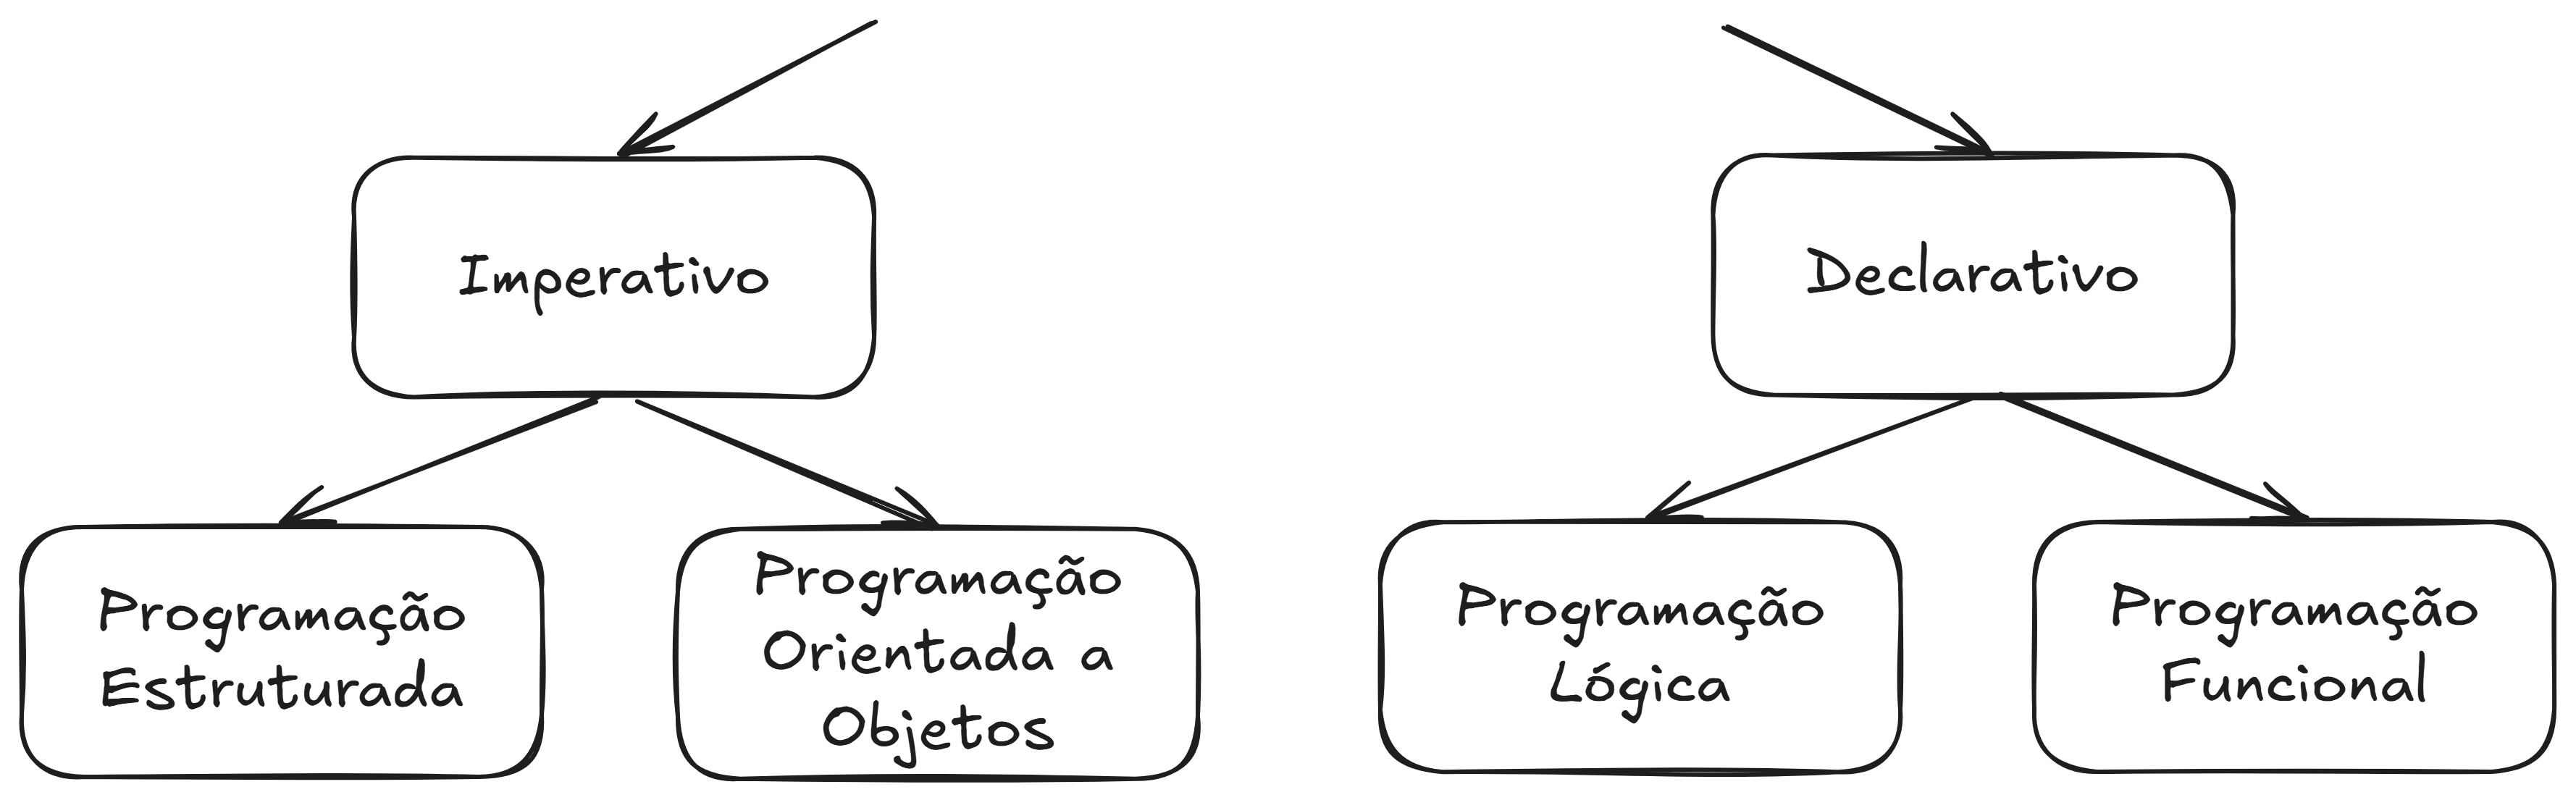
\includegraphics[height=0.17\textheight]{hierarquia_paradigmas}
	\caption{Paradigmas de programação organizados hierarquicamente.}
	\fonte{Adaptado de \citeonline{whatsprogrammingparadigm}.}
	\label{fig:hierarquia_paradigmas}
\end{figure}

Com base na \autoref{fig:hierarquia_paradigmas}, observa-se a relevância dos paradigmas imperativo e declarativo, já que todos os outros paradigmas derivam, em maior ou menor grau, de um desses dois. Por mais que paradigmas mais específicos possam tomar rumos inesperados, eles ainda terão algum grau de herança dos paradigmas imperativo ou declarativo.

Dada a abrangência dos paradigmas imperativo e declarativo, o conhecimento de ambos já se torna suficiente para que o leitor entenda a essência da maioria dos outros paradigmas. Assim, a seguir, eles serão abordados:

\begin{itemize}
	\item \textbf{Paradigma Imperativo}: descreve a aplicação em termos de instruções que alteram o estado do programa, linha por linha. O foco está \textit{em como} fazer algo, geralmente oferecendo maior controle e menor abstração. Exemplos de linguagens imperativas incluem C, Java e Python;
	\item \textbf{Paradigma Declarativo}: descreve a aplicação em termos de declarações que expressam \textit{o que} o programa deve fazer, e não \textit{em como} fazer. Esta abordagem costuma ser mais abstrata, porém com menos controle. Exemplos de linguagens declarativas incluem SQL, Haskell e Lisp.
\end{itemize}

\subsubsection{O \textit{Entity Component System} pode ser considerado um paradigma?}

O padrão \textit{Entity Component System} (ECS) será extremamente crucial em todas as fases do projeto, por isso, é importante entender em que definição ele se encaixa.

Com base na definição de paradigma dada pelo dicionário Merriam-Webster:

\begin{citacao}
	Uma estrutura filosófica e teórica de uma escola ou disciplina científica dentro da qual teorias, leis e generalizações e os experimentos realizados em apoio a elas são formulados (\citeauthor{merriamwebster}, \citeyear{merriamwebster}, tradução nossa).
\end{citacao}

O autor da biblioteca de ECS Flecs, \citeonline{ecsparadigm}, defende que o ECS não é um paradigma:

\begin{citacao}
	Isso não corresponde exatamente ao ECS. Ter pensamentos profundos sobre o ECS não é o mesmo que ter uma estrutura filosófica. Tutoriais, documentação e postagens em blogs não equivalem a “teorias, leis e generalizações”. É seguro dizer que a base teórica para o ECS é, na melhor das hipóteses, instável (\citeauthor{ecsparadigm}, \citeyear{ecsparadigm}, tradução nossa).
\end{citacao}

Seguindo a conclusão de \citeonline{ecsparadigm}, o ECS não será tratado como um paradigma ao decorrer do projeto, mas sim apenas como um padrão de arquitetura.


\subsection{Fundamentos do \textit{Design} de Linguagens de Programação}

Com base em \cite{conceptsoflanguages}, pode-se dizer que o \textit{design} de uma linguagem de programação é a definição da estrutura, do comportamento e dos propósitos da linguagem com base em um conjunto de princípios.

Escolhas de \textit{design} exigem consideração cuidadosa, pois geralmente exigem compromissos entre características desejáveis \cite{conceptsoflanguages}. Um exemplo é a escolha entre uma sintaxe concisa, que pode acelerar a escrita, e uma sintaxe explícita, que pode facilitar a leitura e manutenção do código.

De modo a melhor categorizar o \textit{design} de linguagens de programação, \citeonline{designconceptsinlanguages} propõe a divisão em três categorias principais: sintaxe, semântica e pragmática. A seguir, cada uma delas é descrita de forma resumida com base no mesmo autor:

\begin{itemize}
	\item Sintaxe: a estrutura textual da linguagem, incluindo a definição de suas palavras reconhecidas e a forma como elas podem ser combinadas para formar frases válidas;

	\item Semântica: o significado das frases válidas da linguagem, ou seja, o que elas representam e como são interpretadas pelo sistema;

	\item Pragmática: a implementação interna da linguagem, de tal forma que a semântica não se altere.
\end{itemize}

Essa divisão contribui na separação de preocupações, permitindo que a sintaxe seja definida independentemente da semântica e da pragmática, por exemplo. No caso deste trabalho, a ênfase está na sintaxe e semântica, com a pragmática sendo considerada apenas quando necessário.

\subsubsection{Características do \textit{Design} de Linguagens de Programação}

Todo \textit{design} para uma determinada linguagem de programação busca atender a certos critérios, e para isso, é necessário considerar algumas características importantes \cite{conceptsoflanguages}. Com base nisso, a \autoref{tab:criterios_caracteristicas} ilustra algumas dessas características e quais critérios elas atendem.

\begin{table}[h]
	\centering
	\caption{Critérios do \textit{design} de linguagens de programação e as características que os atendem.}
	{
		\begin{tabular}{lccc}
		\hline
		& \multicolumn{3}{c}{\textbf{Critérios}} \\
		\cline{2-4}
		\textbf{Característica} & \textbf{Legibilidade} & \textbf{Facilidade de Escrita} & \textbf{Confiabilidade} \\
		Simplicidade & x & x & x \\
		Ortogonalidade & x & x & x \\
		Tipos de Dados & x & x & x \\
		\textit{Design} da Sintaxe & x & x & x \\
		Suporte a Abstração & & x & x \\
		Expressividade & & x & x \\
		Checagem de Tipos & & & x \\
		Tratamento de Exceções & & & x \\
		Restrição de \textit{Aliasing} & & & x \\
		\hline
		\end{tabular}
	}
	\fonte{Adaptado de \citeonline{conceptsoflanguages}.}
	\label{tab:criterios_caracteristicas}
\end{table}

A seguir, as características ilustradas na \autoref{tab:criterios_caracteristicas} serão descritas de forma resumida com base em \citeonline{conceptsoflanguages}:

\subsubsubsection{Legibilidade}

\begin{itemize}
	\item a
\end{itemize}

\subsubsubsection{Facilidade de Escrita}

\begin{itemize}
	\item a
\end{itemize}

\subsubsubsection{Confiabilidade}

\begin{itemize}
	\item a
\end{itemize}

\subsubsection{Definição Formal de Sintaxe}

BNF e EBNF.


\subsection{\textit{Entity Component System}}

\textit{Entity Component System} (ECS) é um padrão arquitetural baseado no \textit{design} orientado a dados. Ele surgiu na área de desenvolvimento de jogos, onde há uma grande necessidade de otimização e atualizações frequentes no código. Com o passar do tempo, o padrão ECS começou a ser utilizado em outras áreas, como em simulações físicas \cite{flightdynamics}.

O padrão consiste na separação de dado e lógica de tal forma que as vários entidades da aplicação possam ser compostas de dados reutilizáveis e independentes \cite{ecsfaq}, com as funções sendo direcionadas aos dados, e não às entidades em si. Devido ao desacoplamento gerado por essa separação, o padrão ECS garante alta flexibilidade e modularidade, além do aumento de desempenho gerado pela melhor distribuição de dados na memória \cite{ecsstorageinpics}.

Neste projeto, o padrão ECS será um dos principais fundamentos para o \textit{design} e implementação da linguagem de programação, já que o intuito dela será abstrair ele.

\subsubsection{Os Três Elementos Fundamentais do ECS}

Pode-se dizer que o ECS é separado em três elementos fundamentais: entidades, componentes e sistemas \cite{ecsfaq}. Cada um desses elementos desempenha um papel específico na aplicação:

\begin{itemize}
	\item Entidades: identificadores únicos que representam os vários conceitos de uma aplicação. Sozinhas, as entidades não contêm dados nem funcionalidade;
	\item Componentes: estruturas de dados que armazenam informações específicas. Uma entidade pode ter múltiplos componentes diferentes, definindo suas características;
	\item Sistemas: funções responsáveis por processar sobre entidades com um determinado conjunto de componentes — processo denominado \textit{querying}.
\end{itemize}

Como ilustrado na \autoref{fig:diagrama_ecs}, o estado da aplicação é dado por um conjunto de entidades, cada uma com seus respectivos componentes. Os sistemas são responsáveis pela transformação do estado da aplicação, processando as entidades que possuem os componentes necessários para a execução do sistema.

\begin{figure}[H]
	\centering
	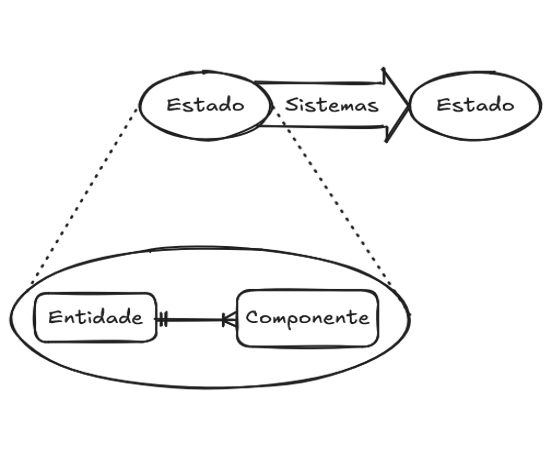
\includegraphics[width=0.35\textheight]{diagrama_ecs}
	\caption{Relação entre entidades, componentes e sistemas.}
	\fonte{Elaboração própria.}
	\label{fig:diagrama_ecs}
\end{figure}

Em termos de código, o padrão ECS pode ser representado sem nenhum construto especializado, mapeando entidades para números únicos, componentes para \textit{structs} e sistemas para funções, como ilustrado no \autoref{cod:exemplo_ecs}.

\codigoRust
\lstinputlisting[
	language=Rust,
	label=cod:exemplo_ecs,
	caption=Implementação simplificada de um padrão ECS incompleto.
]{../codes/exemplo_ecs.rs}
\vspace{-1em}
\fonte{Elaboração própria.}

É importante ressaltar que o \autoref{cod:exemplo_ecs}, por mais que seja funcional e siga o \textit{design} orientado a dados, ainda é uma simplificação da implementação de um padrão ECS incompleto. Na prática, o armazenamento dos dados é feito através de estruturas de dados mais complexas \cite{ecsstorageinpics}, que permitem que entidades escolham quais componentes possuem, que sistemas sejam executados automaticamente, além de outras funcionalidades principais do padrão ECS.

Fora a definição de ECS e seus três elementos fundamentais, o padrão ainda peca pela falta de formalização — quais são as práticas recomendadas ao usar ECS? Como os sistemas são executados? E se apenas entidades, componentes e sistemas não forem suficientes para resolver meu problema? Essas perguntas não possuem respostas definitivas, porém, diferentes autores e implementações abordam o padrão do seu jeito. A seguir, são apresentados alguns conceitos herdados de tais autores e implementações.

\subsubsection{Agendador}

O agendador é um construto com a finalidade de executar todos os sistemas da aplicação, podendo determinar a ordem e frequência de execução de forma declarativa, resolvendo dependência entre sistemas e tornando o ciclo de atualização da aplicação mais previsível \cite{bevy}. Pode-se dizer que, dentre os conceitos mais experimentais, o agendador é o mais próximo de uma formalização.

A \autoref{fig:diagrama_agendador} ilustra o agendador executando os sistemas de forma cíclica e sequencial, onde cada sistema é executado uma vez por ciclo. O agendador pode ser configurado para executar sistemas em diferentes momentos do ciclo, como antes ou depois de outros sistemas.

\begin{figure}[H]
	\centering
	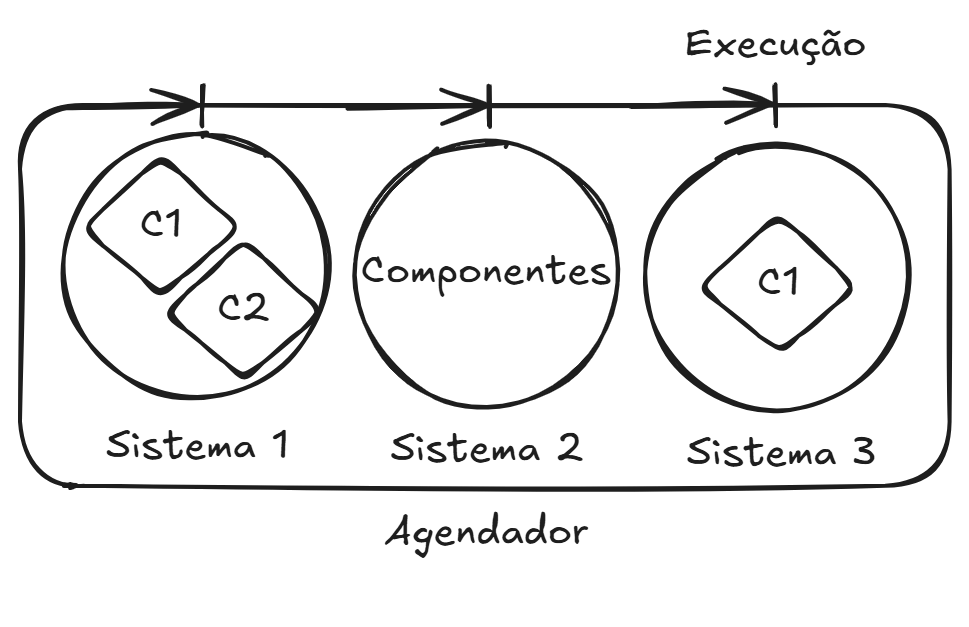
\includegraphics[width=0.3\textheight]{diagrama_agendador}
	\caption{Agendador executando os sistemas de forma cíclica e sequencial.}
	\fonte{Elaboração própria.}
	\label{fig:diagrama_agendador}
\end{figure}

\subsubsection{Relacionamento de Entidades}

Independente da aplicação, é muito comum a necessidade de relacionar diferentes conceitos entre si. Exemplo disso são os sistemas de arquivos, onde pastas podem conter arquivos, uma relação pai-filho.

Relacionamento de entidades (do inglês, \textit{entity relationship}) é um conceito que supre essa necessidade, permitindo que entidades se relacionem entre si. O autor da biblioteca Flecs, \citeonline{flecs}, explica o conceito fazendo uma paralela com o simples ato de adicionar um componente a uma entidade, como ilustrado na \autoref{fig:entidade_posicao}.

\begin{figure}[H]
	\centering
	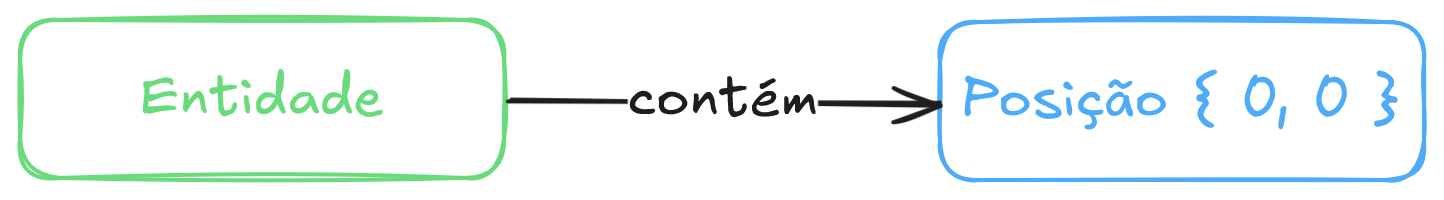
\includegraphics[height=0.06\textheight]{entidade_posicao}
	\caption{Representação do relacionamento entre o Sol, a Terra e a Lua.}
	\fonte{Adaptado de \citeonline{entityrelationships}.}
	\label{fig:entidade_posicao}
\end{figure}

Do mesmo jeito que se adiciona um único componente a uma entidade, como mostra a \autoref{fig:entidade_posicao}, pode-se criar um relacionamento entre duas entidades adicionando uma tupla componente-entidade, onde o componente dita o tipo de relação.

Como exemplo, a \autoref{fig:relacionamento_entidades} ilustra o relacionamento entre o Sol, a Terra e a Lua, onde a Terra é filha do Sol e a Lua é filha da Terra.

\begin{figure}[H]
	\centering
	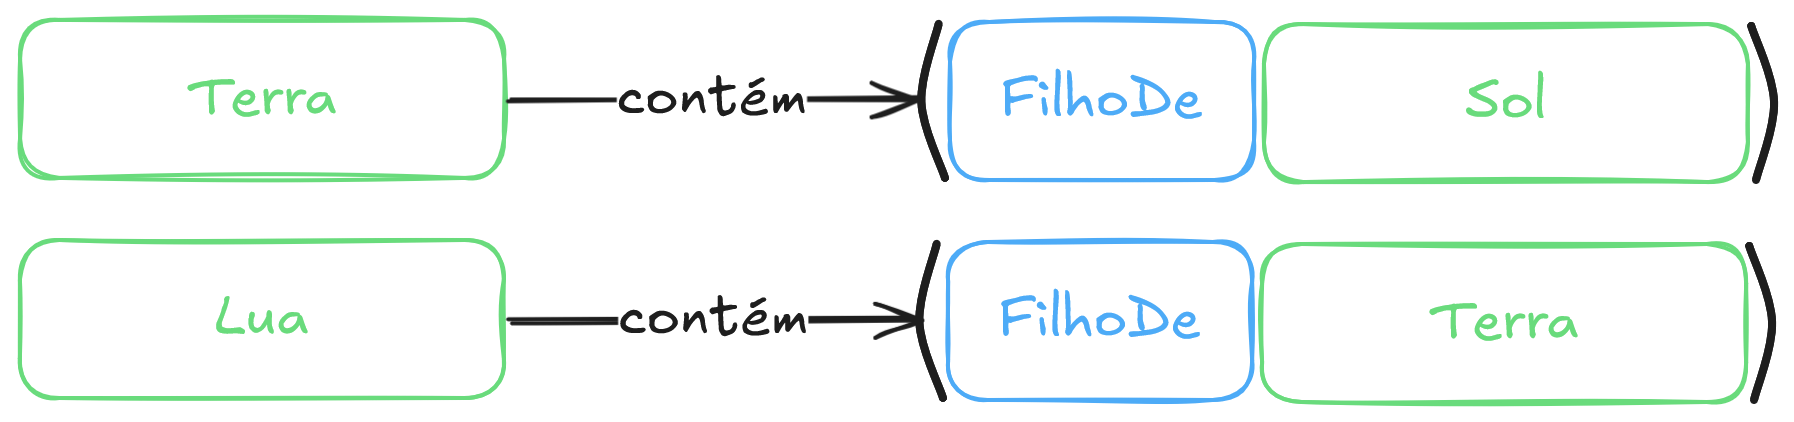
\includegraphics[height=0.13\textheight]{relacionamento_entidades}
	\caption{Representação do relacionamento entre o Sol, a Terra e a Lua.}
	\fonte{Adaptado de \citeonline{entityrelationships}.}
	\label{fig:relacionamento_entidades}
\end{figure}


\subsection{Interpretador \textit{Tree-Walking}}

Um interpretador é um programa que executa diretamente o código fonte de uma linguagem de programação, linha por linha. No caso deste trabalho, será utilizada a variante \textit{tree-walking}, que simplifica o método de execução do interpretador ao custo de desempenho \cite{craftinginterpreters}. Esta variante se adequa ao objetivo do trabalho, que visa a implementação de um protótipo simples, sem preocupações com desempenho.

A \autoref{fig:mapa_interpretador} ilustra uma montanha fazendo analogia a alguns dos principais caminhos que a implementação de uma linguagem de programação pode seguir. Como será implementado um interpretador \textit{tree-walking} neste trabalho, o caminho pela montanha será o da fase de análise léxica, análise sintática, análise semântica e, por fim, evitando a descida pela montanha, a interpretação direta da representação intermediária gerada pela análise semântica.

\begin{figure}[H]
	\centering
	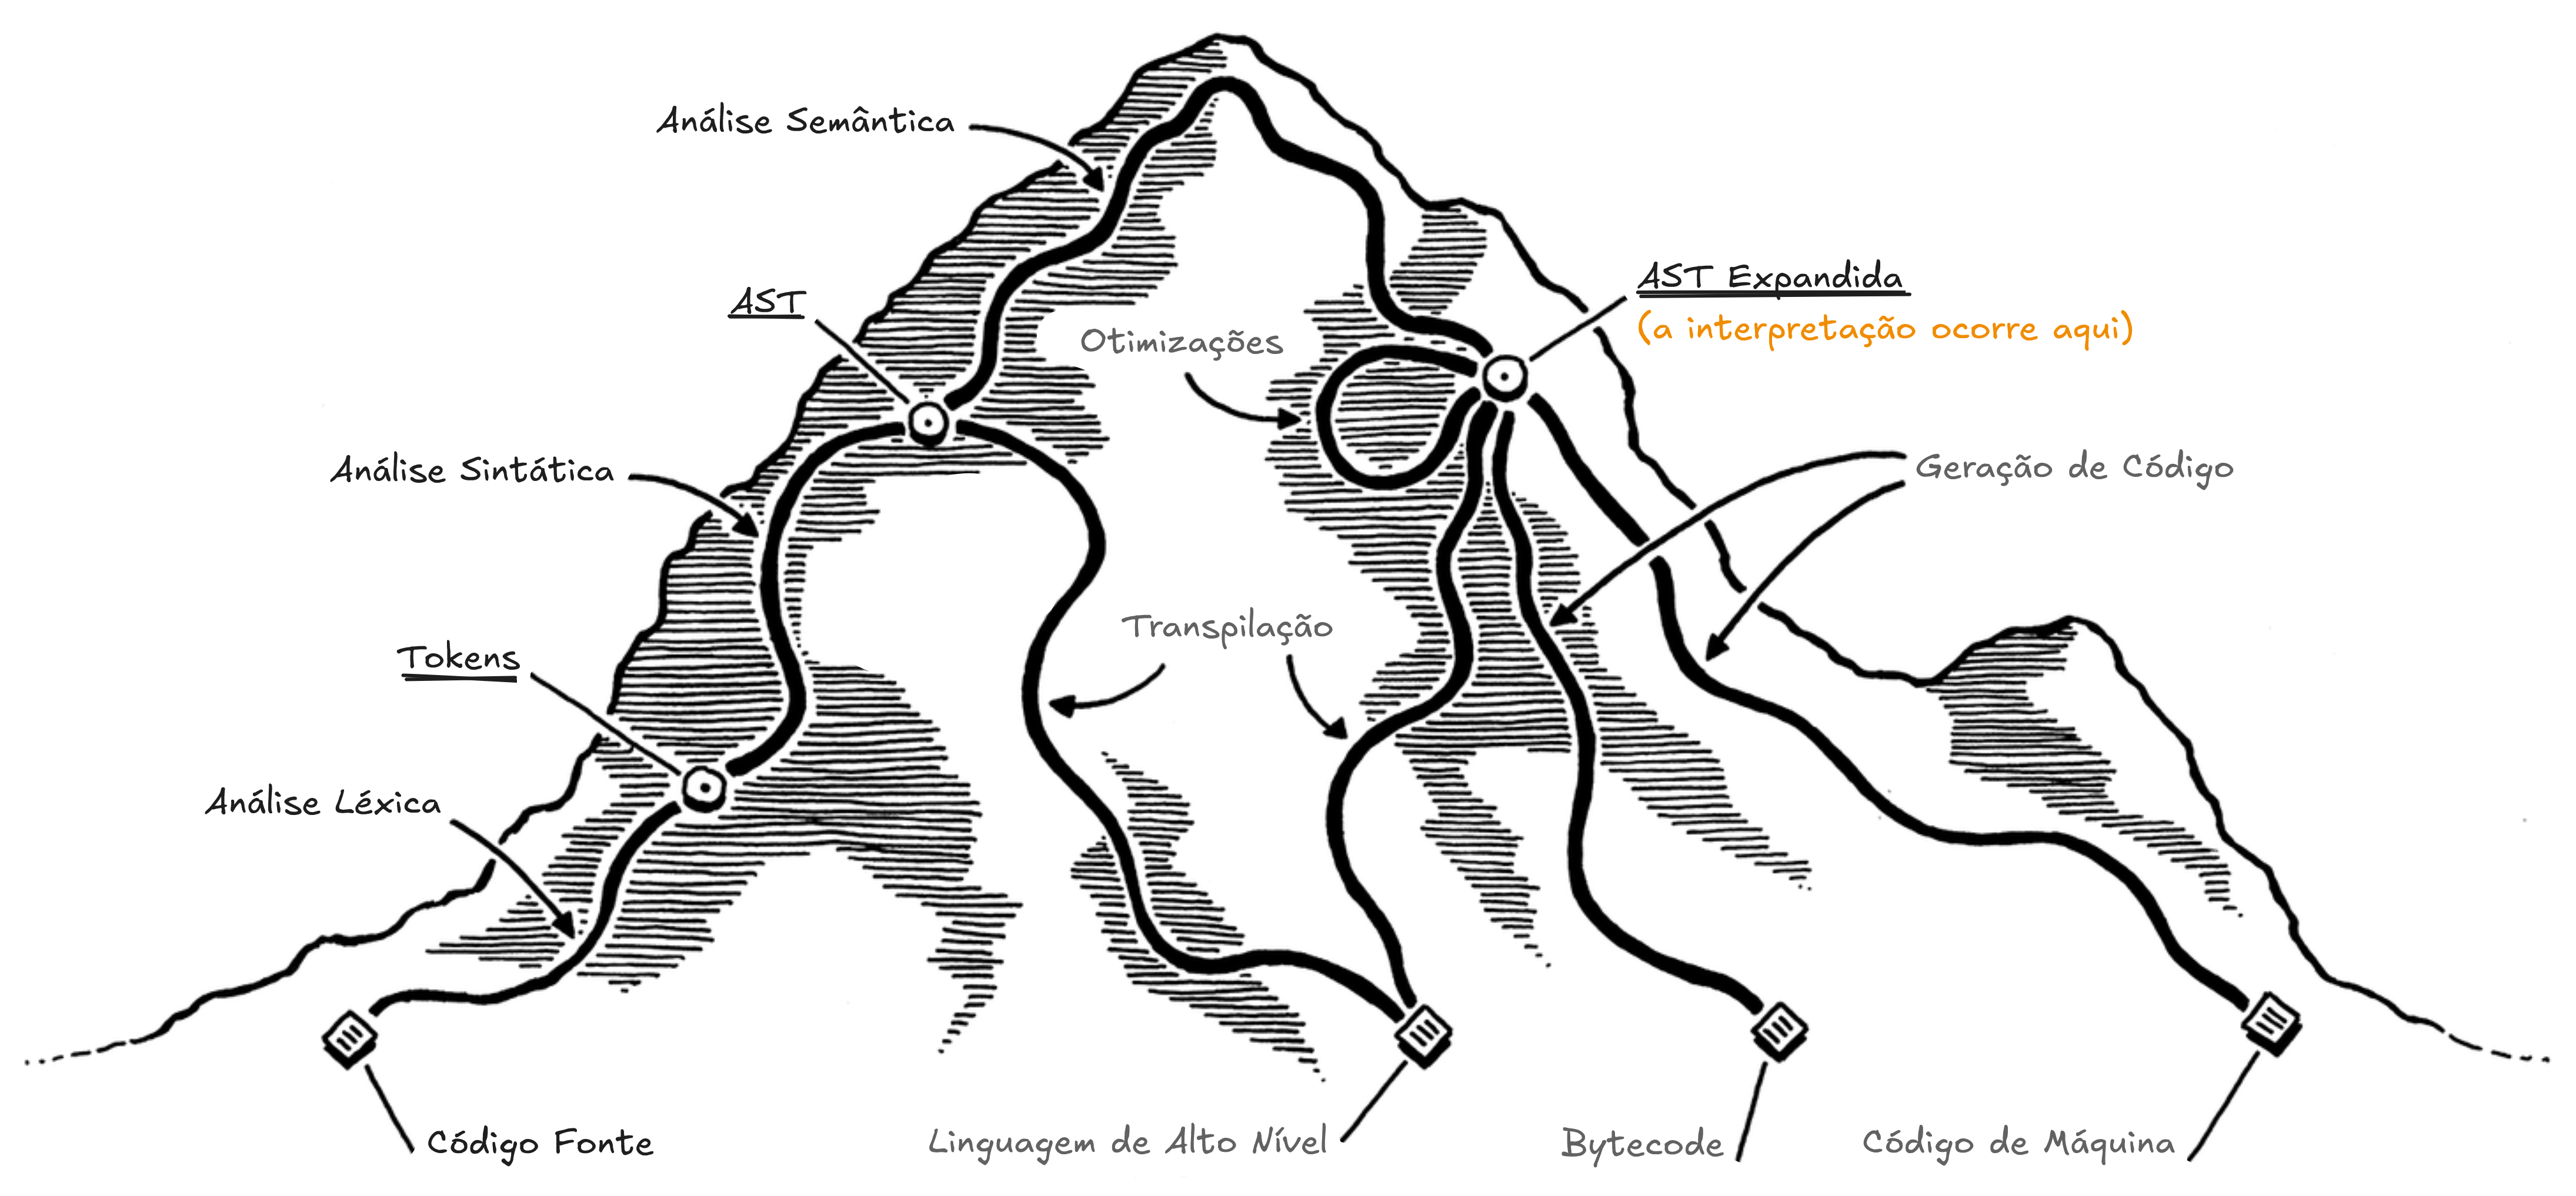
\includegraphics[height=0.275\textheight]{mapa_interpretador}
	\caption{Mapa do território de um interpretador.}
	\fonte{\cite{craftinginterpreters}.}
	\label{fig:mapa_interpretador}
\end{figure}

A seguir, serão definidas em detalhe cada uma das quatro principais fases de um interpretador.

\subsubsection{Análise Léxica}

A análise léxica, também conhecida como \textit{lexer}, é a primeira fase do processo de interpretação. Nesta fase, o código fonte é lido e dividido em unidades chamadas \textit{tokens}. Cada \textit{token} representa uma palavra ou símbolo da linguagem de programação, como palavras-chave e operadores. Além disso, cada \textit{token} costuma conter informações adicionais a respeito da palavra, como sua localização ou valor agregado, caso ela possua algum \cite{craftinginterpreters}.

A \autoref{fig:analise_lexica} ilustra o código fonte \texttt{8 + 4 / 2} sendo mapeado para uma lista de \textit{tokens}, onde cada um representa sua determinada palavra do código fonte.

\begin{figure}[H]
	\centering
	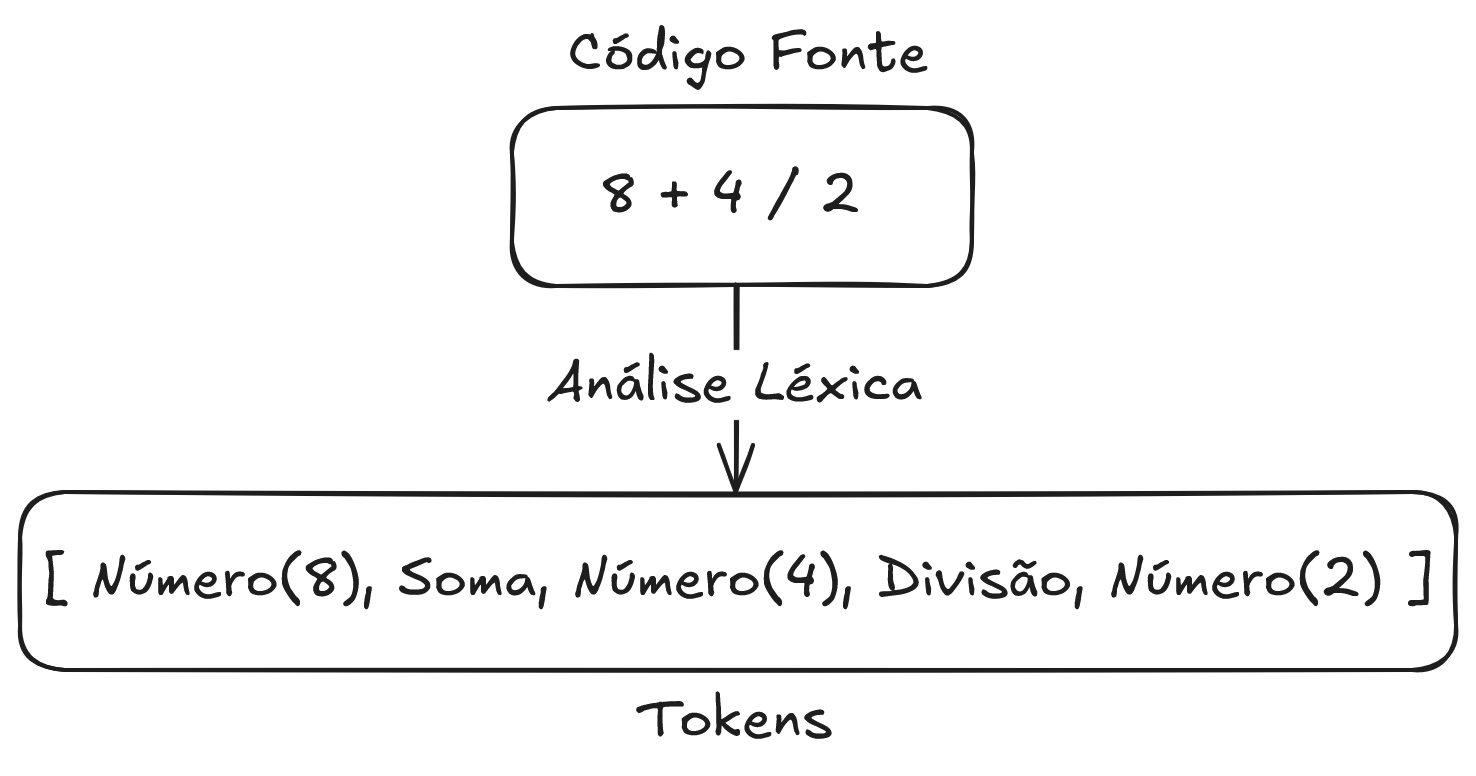
\includegraphics[height=0.2\textheight]{analise_lexica}
	\caption{Código fonte sendo mapeado para uma lista de tokens pela análise léxica.}
	\fonte{Elaboração própria com base em \citeonline{craftinginterpreters}.}
	\label{fig:analise_lexica}
\end{figure}

\subsubsection{Análise Sintática}

A análise sintática, também conhecida como \textit{parser}, é a segunda fase do processo de interpretação. Nesta fase, os \textit{tokens} gerados na fase de análise léxica são organizados em uma estrutura hierárquica chamada árvore sintática abstrata (do inglês, \textit{abstract syntax tree} — AST). A AST representa a estrutura do código fonte de acordo com as regras gramaticais da linguagem de programação \cite{craftinginterpreters}.

A \autoref{fig:analise_sintatica} ilustra a lista de \textit{tokens} sendo mapeada para uma AST, assim gerando a ordem de procedência dos operadores.

\begin{figure}[H]
	\centering
	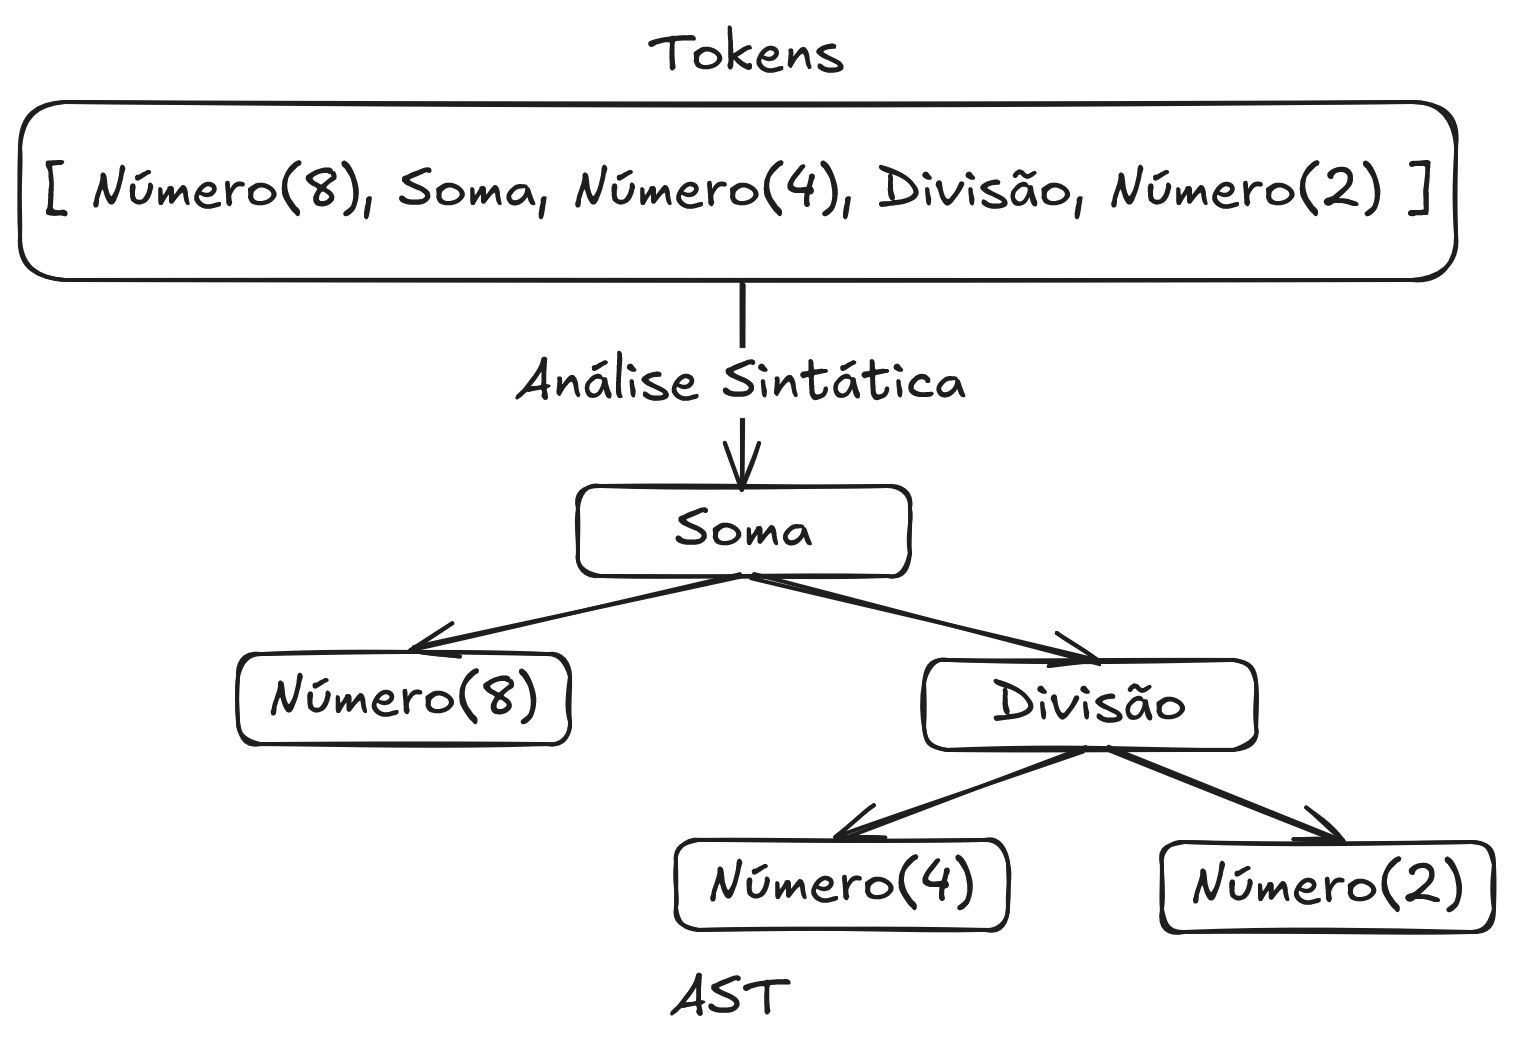
\includegraphics[height=0.27\textheight]{analise_sintatica}
	\caption{Tokens sendo organizados em uma AST pela análise sintática.}
	\fonte{Elaboração própria com base em \citeonline{craftinginterpreters}.}
	\label{fig:analise_sintatica}
\end{figure}

\subsubsection{Análise Semântica}

A análise semântica é uma fase opcional\footnote{Neste trabalho, a análise semântica será implementada.} do processo de interpretação, que visa verificar a consistência e validade do código fonte, além de anotar a AST com informações adicionais, como o tipo de cada expressão \cite{craftinginterpreters}.

Durante esta fase, o interpretador analisa a AST gerada na fase de análise sintática para garantir que as operações e expressões estejam corretas de acordo com as regras da linguagem \cite{craftinginterpreters}. Por exemplo, pode verificar se variáveis foram declaradas antes de serem usadas ou se os tipos de dados são compatíveis.

A \autoref{fig:analise_semantica} ilustra a AST sendo anotada com informações adicionais, como o tipo de cada expressão, resultando em uma AST com mais conhecimento sobre o código fonte.

\begin{figure}[H]
	\centering
	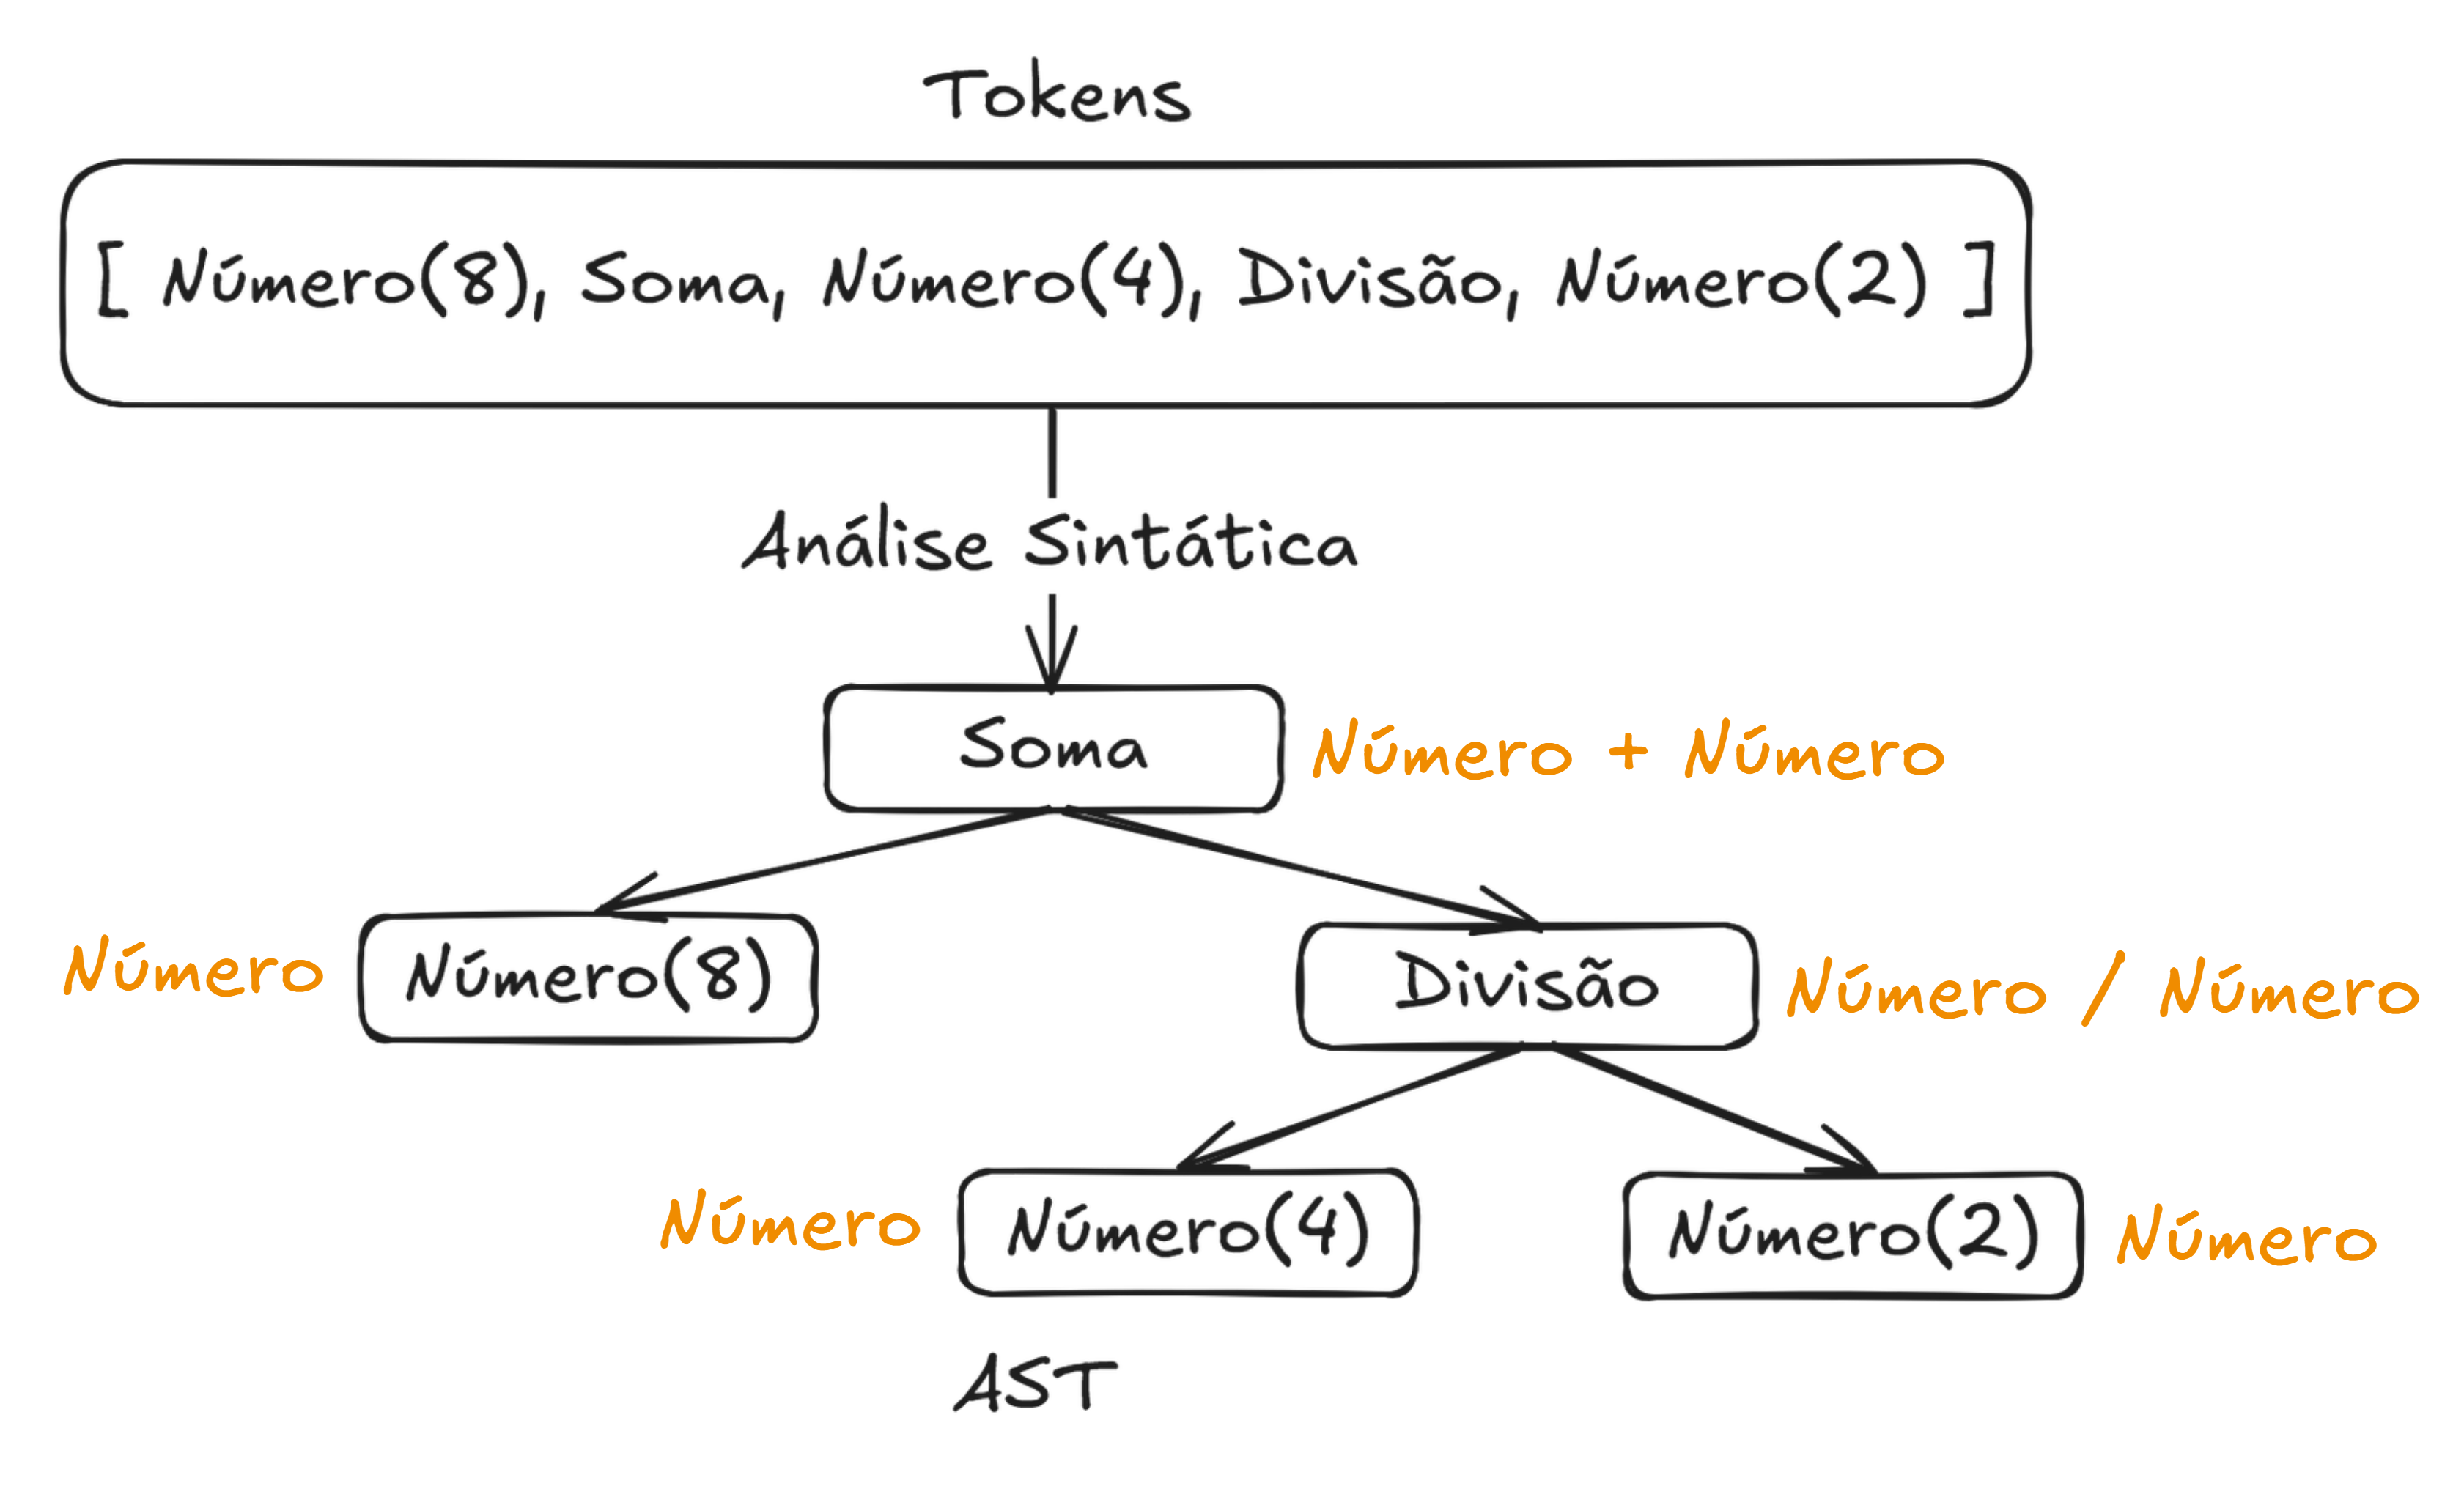
\includegraphics[height=0.27\textheight]{analise_semantica}
	\caption{AST sendo anotada com informações adicionais pela análise semântica.}
	\fonte{Elaboração própria com base em \citeonline{craftinginterpreters}.}
	\label{fig:analise_semantica}
\end{figure}

\subsubsection{Interpretação}

A interpretação é a última fase do processo de interpretação. Nesta fase, a AST gerada na fase de análise sintática e modificada pela análise semântica é percorrida e executada. Durante esta fase, o interpretador avalia expressões, atualiza o estado do programa e executa funções \cite{craftinginterpreters}.

A \autoref{fig:interpretacao} ilustra o processo de interpretação, onde a AST é percorrida e executada pelo interpretador, resultando no número 10.

\begin{figure}[H]
	\centering
	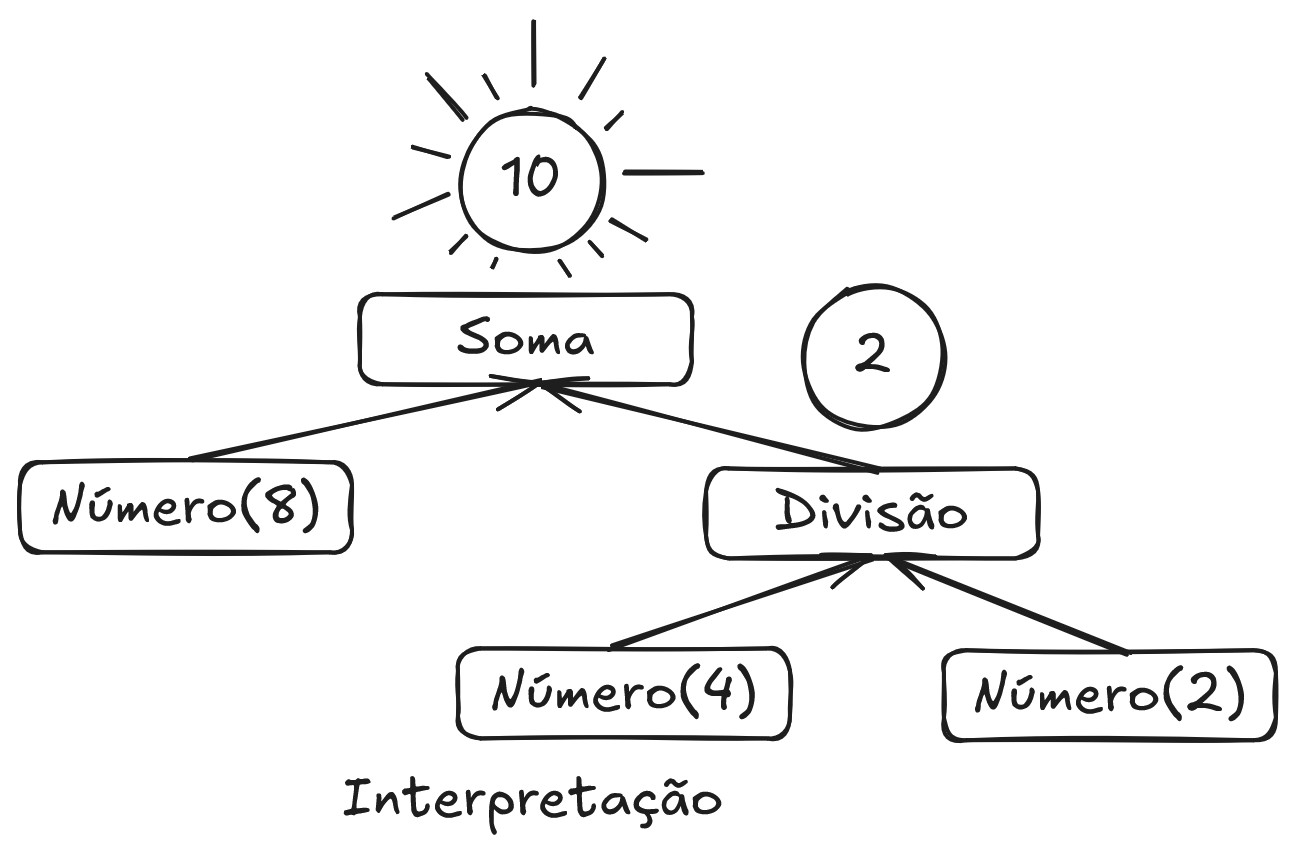
\includegraphics[height=0.25\textheight]{interpretacao}
	\caption{AST sendo percorrida e executada pela fase de interpretação.}
	\fonte{Elaboração própria com base em \citeonline{craftinginterpreters}.}
	\label{fig:interpretacao}
\end{figure}

É importante ressaltar que é na interpretação que o tempo de execução (do inglês, \textit{runtime}) do programa é determinado, pois é quando as expressões são avaliadas e os resultados são produzidos. Em contrapartida, a análise léxica, sintática e semântica são fases de preparação, caracterizando o tempo de compilação (do inglês, \textit{compile time}) do programa.


\section{Tecnologias}

\subsection{Linguagem de Programação Rust}

A linguagem de programação utilizada para o desenvolvimento do interpretador será Rust. A motivação por trás da escolha se dá pelos seguintes fatos:

\begin{itemize}
    \item Possui um sistema de tipagem forte — o uso de enum e match é especialmente útil na definição dos tokens e na construção da AST \cite{rustbook};
    \item O tratamento de erros é explícito, indicando com clareza quais partes do código precisam ser tratadas adequadamente. Todas as fases de um interpretador estão sujeitas a erros, e por isso, tratá-los do jeito mais claro possível é benéfico para o estudo do código \cite{rustbook};
    \item Possui alto desempenho, muitas vezes comparado ao de C. Desempenho é importante não só para ECS em si, mas também para qualquer interpretador, minimizando o tempo que o desenvolvedor espera pela execução de seu código \cite{rustbook}.
\end{itemize}


\subsection{Biblioteca Logos}

Logos é uma biblioteca de análise léxica para Rust. Ela consiste na definição de \textit{tokens} através de \textit{macros} e expressões regulares, tornando o código extremamente conciso.

O \autoref{cod:logos_example} ilustra a definição dos \textit{tokens} de uma calculadora simples, onde cada \textit{token} é definido através de uma expressão regular. A biblioteca automaticamente gera o analisador léxico, que pode ser usado para analisar uma string e retornar os \textit{tokens} correspondentes.

\lstinputlisting[
	language=Rust,
	label=cod:logos_example,
	caption=Análise léxica para uma calculadora usando a biblioteca Logos.
]{../codes/logos_example.rs}
\vspace{-1em}
\fonte{Adaptado de \textcite{logos}.}

Além da simplicidade na definição dos \textit{tokens}, o analisador léxico gerado é extremamente rápido, como mostra o teste de desempenho do repositório oficial da biblioteca na \autoref{tab:logos_benchmark}.

\begin{table}
	\centering
	\caption{Teste de desempenho da biblioteca Logos.}
	{
		\begin{tabular}{ll}
			\hline
			\textbf{Teste} & \textbf{Benchmark} \\ \hline
			Identificadores & 647 ns/iter (+/- 27) = 1204 MB/s \\
			Palavras-chave, operadores e pontuações & 2,054 ns/iter (+/- 78) = 1037 MB/s \\
			Strings & 553 ns/iter (+/- 34) = 1575 MB/s \\ \hline
		\end{tabular}
	}
	\fonte{Adaptado de \textcite{logos}.}
	\label{tab:logos_benchmark}
\end{table}

Por fim, o uso da biblioteca Logos estará na implementação de toda a análise léxica, evitando que tempo seja gasto na análise manual de cada \textit{token}. A motivação para a escolha da biblioteca se deve à sua simplicidade e maturidade no ecossistema Rust, assim minimizando o tempo de desenvolvimento e garantindo maior estabilidade.


\subsection{Biblioteca Chumsky}\label{sec:chumsky}

Chumsky é uma biblioteca de análise sintática para Rust. Ela é baseada no conceito de \textit{parser combinators}\footnote{Um \textit{parser combinator} consiste na combinação de \textit{parsers} mais simples para criar \textit{parsers} mais complexos, assim como é de costume compor uma função maior de funções menores.}, e permite que a definição de \textit{parsers} seja feita de forma declarativa. Seu escopo abrange tanto gramáticas livres de contexto quanto gramáticas sensíveis ao contexto.

Ao usar a biblioteca para construir um \textit{parser}, nota-se a influência do paradigma funcional. Por mais que seja um paradigma mais incomum, seu uso na biblioteca torna o processo de construção do \textit{parser} muito parecido com a construção de uma gramática formal, como demonstrado pelos comentários no \autoref{cod:chumsky_example}.

\codigoRust
\lstinputlisting[
	language=Rust,
	label=cod:chumsky_example,
	caption=\textit{Parser} para uma gramática de expressões aritméticas simples usando a biblioteca Chumsky.
]{../codes/chumsky_example.rs}
\vspace{-1em}
\fonte{Adaptado de \citeonline{chumsky}.}

De acordo com a classificação do teste de desempenho da biblioteca e seus competidores localizada na \autoref{tab:chumsky_benchmark}, Chumsky tem a capacidade de ser a biblioteca de análise sintática mais rápida para Rust.

\FloatBarrier

\begin{table}[H]
	\centering
	\caption{Classificação do teste de desempenho da biblioteca Chumsky e competidores.}
	{
		\begin{tabular}{lll}
			\hline
			\textbf{Classificação} & \textbf{Biblioteca}  & \textbf{Tempo de Execução} \\ \hline
			1                      & chumsky (check-only) & 140.77 µs                  \\
			2                      & winnow               & 178.91 µs                  \\
			3                      & chumsky              & 210.43 µs                  \\
			4                      & sn                   & 237.94 µs                  \\
			5                      & serde\_json          & 477.41 µs                  \\
			6                      & nom                  & 526.52 µs                  \\
			7                      & pest                 & 1.9706 ms                  \\
			8                      & pom                  & 13.730 ms                  \\ \hline
		\end{tabular}
	}
	\fonte{Adaptado de \citeonline{chumsky}.}
	\label{tab:chumsky_benchmark}
\end{table}

Por fim, o uso da biblioteca Chumsky estará na implementação da análise sintática, e será utilizada em conjunto com a biblioteca Logos na implementação do interpretador como um todo. Assim como foi o caso com Logos, a escolha de Chumsky se deve à sua maturidade.

